\documentclass[12pt,a4paper]{article}

% --- Paquetes ---
\usepackage[utf8]{inputenc}
\usepackage[T1]{fontenc}
\usepackage[english]{babel}
\addto\captionsenglish{
  \renewcommand{\contentsname}{Índice}
  \renewcommand{\figurename}{Figura}
  \renewcommand{\tablename}{Tabla}
  \renewcommand{\refname}{Referencias}
}
\usepackage{lmodern}
\usepackage{geometry}
\geometry{margin=2.5cm}
\usepackage{fancyhdr}
\usepackage{amsmath}
\usepackage{graphicx}
\usepackage{float}
\usepackage{booktabs}
\usepackage{array}
\usepackage{xcolor}
\usepackage{listings}
\usepackage{titlesec}
\usepackage{hyperref}
\usepackage{enumitem}
\usepackage{caption}
\usepackage{subcaption}
\usepackage{parskip}

% --- Colores UPS ---
\definecolor{salesiana}{RGB}{0,84,166}
\definecolor{accentgreen}{RGB}{34,139,34}
\definecolor{accentorange}{RGB}{204,85,0}
\definecolor{codebg}{RGB}{245,245,245}

% --- Código ---
\lstdefinestyle{cppstyle}{
  backgroundcolor=\color{codebg},
  basicstyle=\ttfamily\footnotesize,
  keywordstyle=\color{salesiana}\bfseries,
  commentstyle=\color{accentgreen}\itshape,
  stringstyle=\color{accentorange},
  breaklines=true,
  frame=single,
  rulecolor=\color{gray!40},
  numbers=left,
  numberstyle=\tiny\color{gray},
  language=C++,
  literate={á}{{\'a}}1 {é}{{\'e}}1 {í}{{\'i}}1 {ó}{{\'o}}1 {ú}{{\'u}}1
           {ñ}{{\~n}}1 {Á}{{\'A}}1 {É}{{\'E}}1 {Í}{{\'I}}1 {Ó}{{\'O}}1
           {Ú}{{\'U}}1 {Ñ}{{\~N}}1
}
\lstset{style=cppstyle}

% --- Títulos ---
\titleformat{\section}{\large\bfseries\color{salesiana}}{}{0em}{}[\titlerule]
\titleformat{\subsection}{\normalsize\bfseries\color{salesiana!80}}{}{0em}{}

% --- Encabezado/pie ---
\pagestyle{fancy}
\fancyhf{}
\lhead{\small\color{gray}Universidad Politécnica Salesiana}
\rhead{\small\color{gray}Visión por Computador · Práctica 3-1 · 3-2}
\cfoot{\thepage}
\renewcommand{\headrulewidth}{0.4pt}

\hypersetup{colorlinks=true, linkcolor=salesiana, urlcolor=salesiana, citecolor=salesiana}

% =============================================================================
\begin{document}
% =============================================================================

% --- Portada ---
\begin{titlepage}
  \centering
  \rule{\linewidth}{1.5pt}\\[0.4cm]
  {\large\bfseries UNIVERSIDAD POLITÉCNICA SALESIANA}\\[0.1cm]
  {\normalsize CARRERA DE INGENIERÍA EN CIENCIAS DE LA COMPUTACIÓN}\\[0.2cm]
  \rule{\linewidth}{0.8pt}

  \vspace{2cm}

  \parbox{0.85\textwidth}{\centering\LARGE\bfseries\color{salesiana}
    Análisis Comparativo de Robustez entre Momentos de Hu, Zernike
    y Shape Signature, y Reconocimiento de Hojas (Flavia) mediante
    Descriptores de Fourier de Coordenadas Complejas
  }

  \vspace{1.5cm}

  {\large\bfseries Informe de Práctica 3-1 · 3-2 — Visión por Computador (G3)}\\[0.2cm]
  {\normalsize Práctica de Laboratorio — Unidad 3}

  \vspace{1.5cm}

  \begin{tabular}{ll}
    \textbf{Autores:}    & Michael Lata (Lata Zambrano Michael Israel) \\
                         & Jordy Romero (Romero Armijos Jordy Jasmany) \\[0.3cm]
    \textbf{Grupo:}      & G3 — Clases asignadas: 14, 15, 16, 17, 18, 19, 20 \\[0.3cm]
    \textbf{Docente:}    & Vladimir Robles Bykbaev \\[0.3cm]
    \textbf{Asignatura:} & Visión por Computador \\[0.3cm]
    \textbf{Período:}    & Marzo -- Agosto 2026 \\[0.3cm]
    \textbf{Fecha:}      & 24 de junio de 2026 \\
  \end{tabular}

  \vfill
  \rule{\linewidth}{1.5pt}
\end{titlepage}

% --- Resumen ---
\section*{Resumen}

En esta práctica desarrollamos dos sistemas de reconocimiento de formas basados en descriptores globales, sin usar aprendizaje profundo ni redes neuronales. En la \textbf{Parte 1} construimos un cuaderno en Python que compara la robustez de tres descriptores —\textbf{Momentos de Hu}, \textbf{Momentos de Zernike} y \textbf{Shape Signature}— frente a ruido sintético (Gaussiano y Sal \& Pimienta en tres niveles) y rotaciones aleatorias de 0° a 360°, sobre el dataset \textit{UPS-Writing-Skills} (círculo, triángulo, cuadrado). En la \textbf{Parte 2} implementamos una aplicación Android con una \textbf{librería nativa en C++} (vía JNI) que reconoce la especie de una hoja del \textit{Flavia Dataset} usando el descriptor de Fourier de \textbf{coordenadas complejas} $s(n)=(x-x_c)+j(y-y_c)$.

Los resultados confirman la hipótesis de la guía: los Momentos de Hu se quedan en $\sim$64\% de exactitud, mientras que Zernike y Shape Signature alcanzan $\sim$82\% y $\sim$88\% respectivamente, siendo claramente más robustos al ruido. La app móvil, validada en una tablet física, clasifica las 7 clases asignadas al grupo (14--20) con una exactitud del \textbf{93.5\%} y muestra en pantalla la etiqueta de la especie junto a su descriptor de Fourier.

\clearpage
\tableofcontents
\clearpage

% =============================================================================
\section{Introducción}
% =============================================================================

El objetivo de esta práctica es evaluar y comparar \textit{descriptores globales de forma}, que son funciones que resumen una figura completa en un vector de números (un ``descriptor'') invariante a transformaciones como rotación, escala o traslación. La idea central es que dos figuras de la misma clase deberían producir descriptores parecidos aunque estén rotadas o tengan ruido.

Trabajamos con dos enfoques complementarios. El primero son los \textbf{momentos} (Hu y Zernike), que integran toda la región de la figura ponderada por polinomios. El segundo es la \textbf{firma de la forma} (Shape Signature) y su variante de \textbf{coordenadas complejas}, que en lugar de mirar la región completa tratan el \textit{contorno} como una señal y la analizan con la Transformada de Fourier.

Un punto importante de la práctica es que \textbf{no usamos redes neuronales ni aprendizaje profundo}. Todo se resuelve con matemática clásica de visión por computador (OpenCV, NumPy, SciPy, Scikit-Learn), de modo que cada paso es explicable y defendible con el material de la asignatura. La Parte 2 además exige llevar esa matemática a un \textbf{dispositivo móvil real}, lo que añade el reto de implementar los cálculos en C++ y conectarlos con la interfaz Android mediante JNI.

\subsection*{Parámetros personalizados del grupo}

La práctica asignó parámetros personalizados que usamos de forma consistente en todo el proyecto:
\begin{itemize}
  \item \textbf{Umbral de binarización} $T = 130$: separa la tinta del fondo en la segmentación.
  \item \textbf{Vecinos del clasificador} $K = 7$: número de vecinos del KNN.
  \item \textbf{Clases asignadas (G3):} 14, 15, 16, 17, 18, 19, 20 del Flavia Dataset.
\end{itemize}

% =============================================================================
\section*{Repositorios del Proyecto}
% =============================================================================

\begin{itemize}
  \item \textbf{Repositorio del proyecto (Parte 1 + Parte 2 + App Android):}\\
        \url{https://github.com/USUARIO/REPO}  % <-- reemplazar por el enlace real del repo
\end{itemize}

\textit{Nota: el repositorio contiene el cuaderno de la Parte 1 (\texttt{notebooks/}), el núcleo C++ compartido (\texttt{cpp/}), la app Android (\texttt{mobile/}), los scripts de orquestación (\texttt{scripts/}) y los resultados (\texttt{results/}).}

% =============================================================================
\section{Parte 1: Robustez de Hu vs. Zernike vs. Shape Signature}
% =============================================================================

\subsection{Dataset y preprocesamiento}

Usamos el dataset \textit{UPS-Writing-Skills}, que contiene trazos hechos a mano de tres figuras geométricas: \textbf{círculo}, \textbf{triángulo} y \textbf{cuadrado}. Como son dibujos a mano alzada, los trazos a veces quedan abiertos o con huecos, así que la segmentación no puede ser un simple umbral.

Nuestra solución fue binarizar con el umbral $T=130$ y luego tomar la \textbf{envolvente convexa} (\textit{convex hull}) de la tinta significativa. Las tres clases son figuras convexas, así que el \textit{convex hull} reconstruye una silueta sólida y cerrada incluso cuando el trazo original tiene huecos. Esto evita que un dibujo abierto genere un contorno roto que arruine los descriptores.

\begin{lstlisting}
# Binarizacion con el umbral personalizado T=130 + filtro de mediana
_, binaria = cv2.threshold(gris, T_THRESHOLD, 255, cv2.THRESH_BINARY_INV)
binaria = cv2.medianBlur(binaria, MEDIAN_KSIZE)  # robusto a Sal & Pimienta
# Envolvente convexa de la tinta significativa -> silueta solida
hull = cv2.convexHull(np.vstack(componentes_significativos))
\end{lstlisting}

El filtro de mediana antes de extraer los momentos es justamente la recomendación de la guía para mitigar el ruido Sal \& Pimienta, que de otro modo distorsiona el cálculo del centroide.

\subsection{Inyección de ruido y aumento de datos}

Implementamos una función de inyección de ruido con dos tipos y tres niveles de intensidad (bajo, medio, alto), tal como pide la guía:

\textbf{Ruido Gaussiano} — se suma a cada píxel un valor de una distribución normal:
\[
I_{\text{salida}}(x,y) = I(x,y) + \mathcal{N}(0,\,\sigma^2)
\]

\textbf{Ruido Sal \& Pimienta} — se ponen aleatoriamente píxeles en blanco (sal) o negro (pimienta) con probabilidad $p$ (0.02, 0.06 y 0.12 para bajo, medio y alto).

Además, para cada imagen generamos varias \textbf{rotaciones aleatorias de 0° a 360°}. Esto es clave: si un descriptor es realmente invariante a la rotación, su exactitud no debería caer al introducir estas rotaciones.

\subsection{Extracción de los tres descriptores}

\textbf{Momentos de Hu.} Calculamos los 7 momentos invariantes de Hu y les aplicamos la transformación logarítmica vista en clase para que todos queden en órdenes de magnitud comparables:
\[
h'_i = -\,\text{sign}(h_i)\cdot \log_{10}(|h_i|)
\]

\textbf{Momentos de Zernike.} Los implementamos \textit{desde cero} (no hay función directa en OpenCV) con grado de polinomio $n=8$. Se construye la base compleja $V_{nm}(\rho,\theta)=R_{nm}(\rho)\,e^{jm\theta}$ sobre el disco unitario y se proyecta la imagen sobre ella; usamos las \textbf{magnitudes} $|A_{nm}|$ porque son invariantes a la rotación (una rotación solo cambia la fase). Esto da 25 descriptores para $n=8$.

\textbf{Shape Signature.} Calculamos la firma de distancia al centroide del contorno, le aplicamos la FFT y nos quedamos con los \textbf{13 primeros componentes de frecuencia}: el primero (DC) normaliza y los 12 siguientes forman el descriptor, exactamente como indica la guía.

\subsection{Clasificación y prevención de fuga de datos}

Entrenamos un clasificador \textbf{KNN con $K=7$} para cada descriptor. Un detalle metodológico importante: como generamos varias variantes (rotadas/ruidosas) de la \textit{misma} imagen original, usamos \texttt{GroupShuffleSplit} para que todas las variantes de una imagen caigan juntas en \textit{train} o en \textit{test}, nunca repartidas. Si no se hace esto, el modelo ``ve'' en entrenamiento una versión casi idéntica de lo que luego evalúa, e infla artificialmente la exactitud (fuga de datos).

\subsection{Resultados}

La Tabla~\ref{tab:robustez} resume la exactitud de cada descriptor por nivel de ruido, y las Figuras~\ref{fig:robustez} y~\ref{fig:cm_p1} lo muestran gráficamente.

\begin{table}[htbp]
  \centering
  \caption{Exactitud (accuracy) por descriptor y nivel de ruido. KNN con $K=7$.}
  \begin{tabular}{llcccc}
    \toprule
    \textbf{Ruido} & \textbf{Descriptor} & \textbf{Limpio} & \textbf{Bajo} & \textbf{Medio} & \textbf{Alto} \\
    \midrule
    Gaussiano      & Hu              & 0.645 & 0.623 & 0.606 & 0.651 \\
    Gaussiano      & Zernike         & 0.822 & 0.822 & 0.814 & 0.842 \\
    Gaussiano      & Shape Signature & 0.830 & 0.792 & 0.848 & \textbf{0.888} \\
    \midrule
    Sal \& Pimienta & Hu              & 0.645 & 0.652 & 0.634 & 0.606 \\
    Sal \& Pimienta & Zernike         & 0.822 & 0.826 & 0.835 & 0.759 \\
    Sal \& Pimienta & Shape Signature & 0.830 & 0.855 & \textbf{0.867} & 0.795 \\
    \bottomrule
  \end{tabular}
  \label{tab:robustez}
\end{table}

\begin{figure}[htbp]
  \centering
  \begin{subfigure}[b]{0.49\textwidth}
    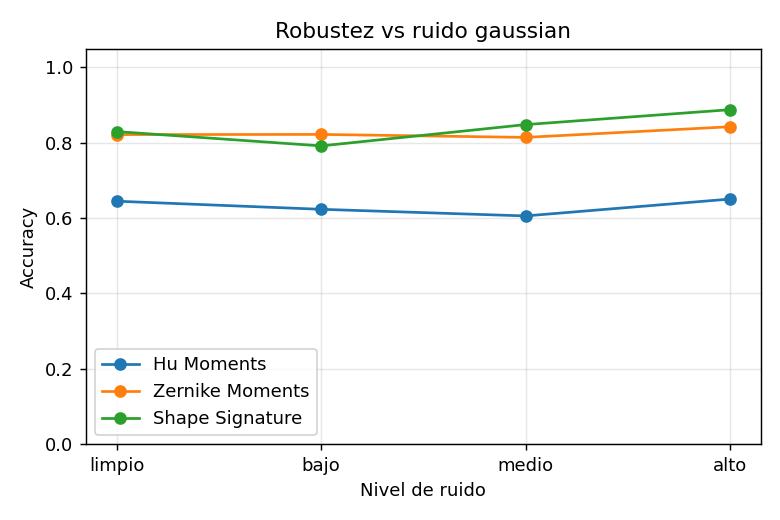
\includegraphics[width=\textwidth]{figuras/robustez_gaussian.png}
    \caption{Ruido Gaussiano}
  \end{subfigure}
  \hfill
  \begin{subfigure}[b]{0.49\textwidth}
    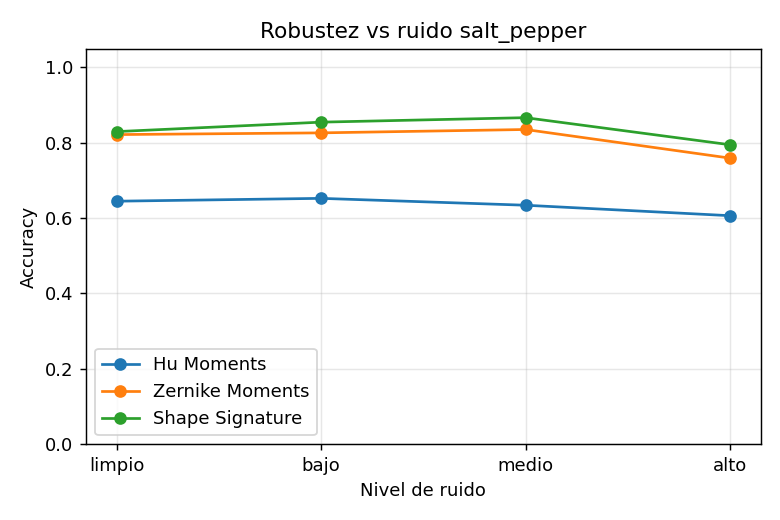
\includegraphics[width=\textwidth]{figuras/robustez_salt_pepper.png}
    \caption{Ruido Sal \& Pimienta}
  \end{subfigure}
  \caption{Curvas de robustez: exactitud frente al nivel de ruido. Hu (azul) se mantiene muy por debajo de Zernike (naranja) y Shape Signature (verde) en todos los niveles.}
  \label{fig:robustez}
\end{figure}

El resultado es claro y coincide con la conclusión esperada por la guía (``superioridad de la ortogonalidad''): los \textbf{Momentos de Hu} apenas superan el 60\%, mientras que \textbf{Zernike} y \textbf{Shape Signature} se mantienen sobre el 80\% incluso con ruido alto. La razón es que Hu solo tiene 7 valores muy redundantes entre sí, mientras que Zernike (base ortogonal) y la firma espectral capturan más detalle de la forma sin redundancia.

\begin{figure}[htbp]
  \centering
  \begin{subfigure}[b]{0.32\textwidth}
    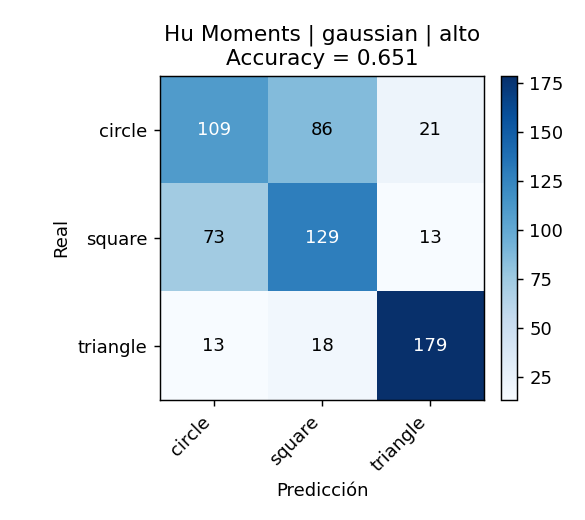
\includegraphics[width=\textwidth]{figuras/cm_gaussian_alto_hu.png}
    \caption{Hu — ruido alto}
  \end{subfigure}
  \hfill
  \begin{subfigure}[b]{0.32\textwidth}
    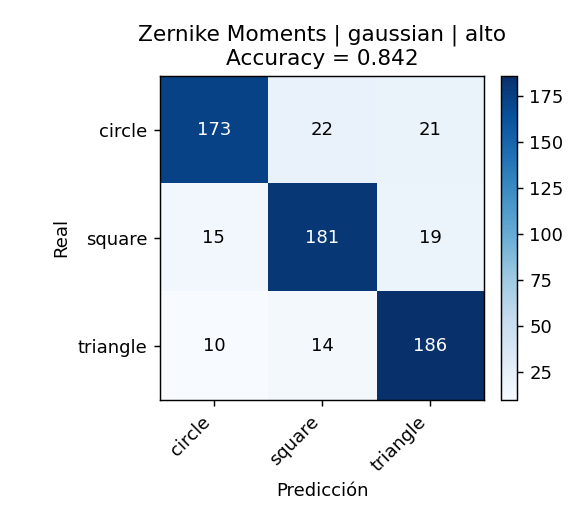
\includegraphics[width=\textwidth]{figuras/cm_gaussian_alto_zernike.png}
    \caption{Zernike — ruido alto}
  \end{subfigure}
  \hfill
  \begin{subfigure}[b]{0.32\textwidth}
    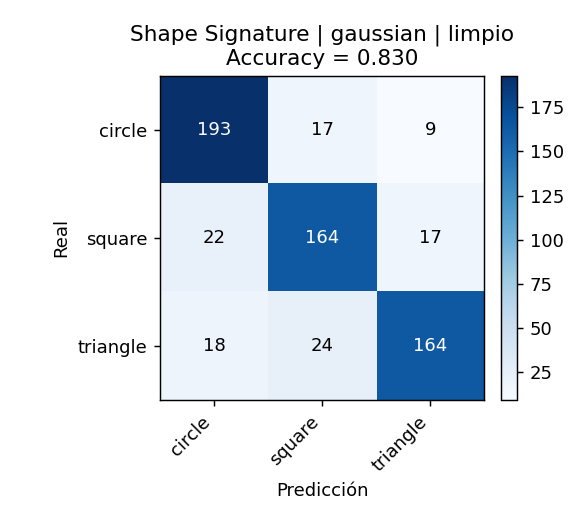
\includegraphics[width=\textwidth]{figuras/cm_gaussian_limpio_shape_signature.png}
    \caption{Shape Sig. — limpio}
  \end{subfigure}
  \caption{Matrices de confusión por descriptor (se generó una por cada nivel de ruido). En Hu el triángulo y el cuadrado se confunden mucho; Zernike y Shape Signature separan mejor las tres clases.}
  \label{fig:cm_p1}
\end{figure}

\begin{figure}[htbp]
  \centering
  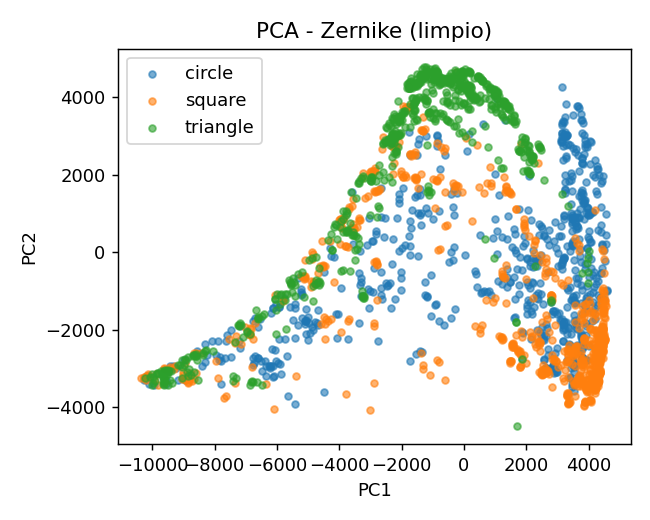
\includegraphics[width=0.7\textwidth]{figuras/pca_zernike_limpio.png}
  \caption{Proyección PCA de los descriptores de Zernike (datos limpios). Se observa cómo las tres clases forman grupos relativamente separados; al añadir ruido estos clusters se ``mezclan'', lo que explica la caída de exactitud.}
  \label{fig:pca}
\end{figure}

% =============================================================================
\section{Parte 2: App Android — Reconocimiento de Hojas (Flavia)}
% =============================================================================

\subsection{Arquitectura: un núcleo C++ compartido}

La guía exige que ``todos los cálculos se realicen en una librería nativa de C++''. Para cumplirlo de forma limpia, escribimos el algoritmo \textbf{una sola vez} en C++ (\texttt{cpp/src/shape\_descriptor.cpp}) y lo compilamos en dos sitios: una CLI de escritorio (para validar y entrenar) y la app Android (vía JNI). Así garantizamos que el móvil y el PC producen \textit{exactamente} el mismo descriptor.

\begin{figure}[htbp]
  \centering
  \fbox{\parbox{0.9\textwidth}{\ttfamily\small
  UI (Java/Android)\hfill Núcleo C++ (JNI)\\
  \rule{\linewidth}{0.3pt}\\
  MainActivity --- botón ---$>$ NativeBridge.nativeClassify(matAddr)\\
  DrawView (lienzo) ---$>$ OpenCV bitmapToMat ---$>$ native\_lib.cpp\\
  \hspace*{4cm}$>$ shape\_descriptor.cpp (cv::dft, |F|/|F(1)|, dist. Euclídea, KNN $K=7$)
  }}
  \caption{Arquitectura de la app: la interfaz en Java captura el dibujo y delega todo el cálculo al núcleo C++ compartido mediante JNI.}
  \label{fig:arq}
\end{figure}

\subsection{Variante matemática: coordenadas complejas y FFT}

En lugar de medir distancias al centroide, tratamos el contorno como una señal en el plano complejo, tal como pide la guía:
\[
s(n) = \big(x(n) - x_c\big) + j\,\big(y(n) - y_c\big)
\]
donde $(x_c, y_c)$ es el centroide. El flujo en tiempo real es:
\begin{enumerate}
  \item \textbf{Segmentación} por umbral adaptativo (el dibujo es trazo oscuro sobre fondo claro).
  \item \textbf{Contorno} externo más grande con \texttt{cv::findContours}.
  \item \textbf{DFT} de la señal compleja con \texttt{cv::dft} y \texttt{DFT\_COMPLEX\_OUTPUT}.
  \item \textbf{Normalización} dividiendo por $|F(1)|$ (invarianza a escala) y descartando la fase (invarianza a rotación).
\end{enumerate}

\begin{lstlisting}
// Senal compleja s(n) = (x - xc) + j (y - yc)  -> Mat N x 1, 2 canales
cv::Mat signal(nPoints, 1, CV_32FC2);
for (int i = 0; i < nPoints; ++i)
    signal.at<cv::Vec2f>(i, 0) =
        cv::Vec2f(pts[i].x - c.x, pts[i].y - c.y);

cv::Mat spectrum;
cv::dft(signal, spectrum, cv::DFT_COMPLEX_OUTPUT);  // FFT compleja

// Normalizar por |F(1)| y descartar fase (solo magnitudes)
float f1 = std::max(mag[1], mag[nPoints - 1]);
for (int k = 0; k < nDescriptors; ++k)
    desc.push_back(mag[k] / f1);
\end{lstlisting}

\textbf{Un detalle no obvio que tuvimos que corregir.} \texttt{cv::findContours} a veces devuelve el contorno en sentido \textit{horario}, lo que coloca el armónico fundamental en $F(N-1)$ en lugar de $F(1)$. Cuando eso pasa, $|F(1)|\approx 0$ y al dividir por él el descriptor ``explota'' (valores enormes y distancias absurdas). La solución fue forzar la orientación \textbf{antihoraria} calculando el área con signo y, si es negativa, invertir el contorno. Tras esta corrección, el descriptor de una figura y el de su versión rotada/escalada quedan prácticamente idénticos (distancia $<0.001$).

\subsection{Entrenamiento y clasificación}

Dividimos el dataset en \textbf{80\% train / 20\% test por cada clase}. Para clasificar comparamos el descriptor de la imagen de prueba con los de entrenamiento usando \textbf{distancia Euclídea} (la misma métrica vista en el tema de Momentos de Hu) y un voto KNN con $K=7$. Los descriptores de entrenamiento de las 7 clases (350 muestras) se empaquetan en \texttt{assets/model.csv} dentro del APK.

\subsection{La aplicación funcionando en la tablet}

La app presenta un área de dibujo y un botón ``Clasificar forma''. Al pulsarlo, toma el lienzo, lo convierte a \texttt{cv::Mat} y llama al núcleo C++, que devuelve la especie y los primeros valores del descriptor. La Figura~\ref{fig:app} muestra la app ejecutándose en una tablet física (modelo 9185W, Android~15): se dibujó una hoja lanceolada y el sistema respondió \textbf{``ESPECIE CLASIFICADA: 19''} junto con su descriptor de Fourier, exactamente en el formato de la Ilustración~3 de la guía.

\begin{figure}[htbp]
  \centering
  \begin{subfigure}[b]{0.42\textwidth}
    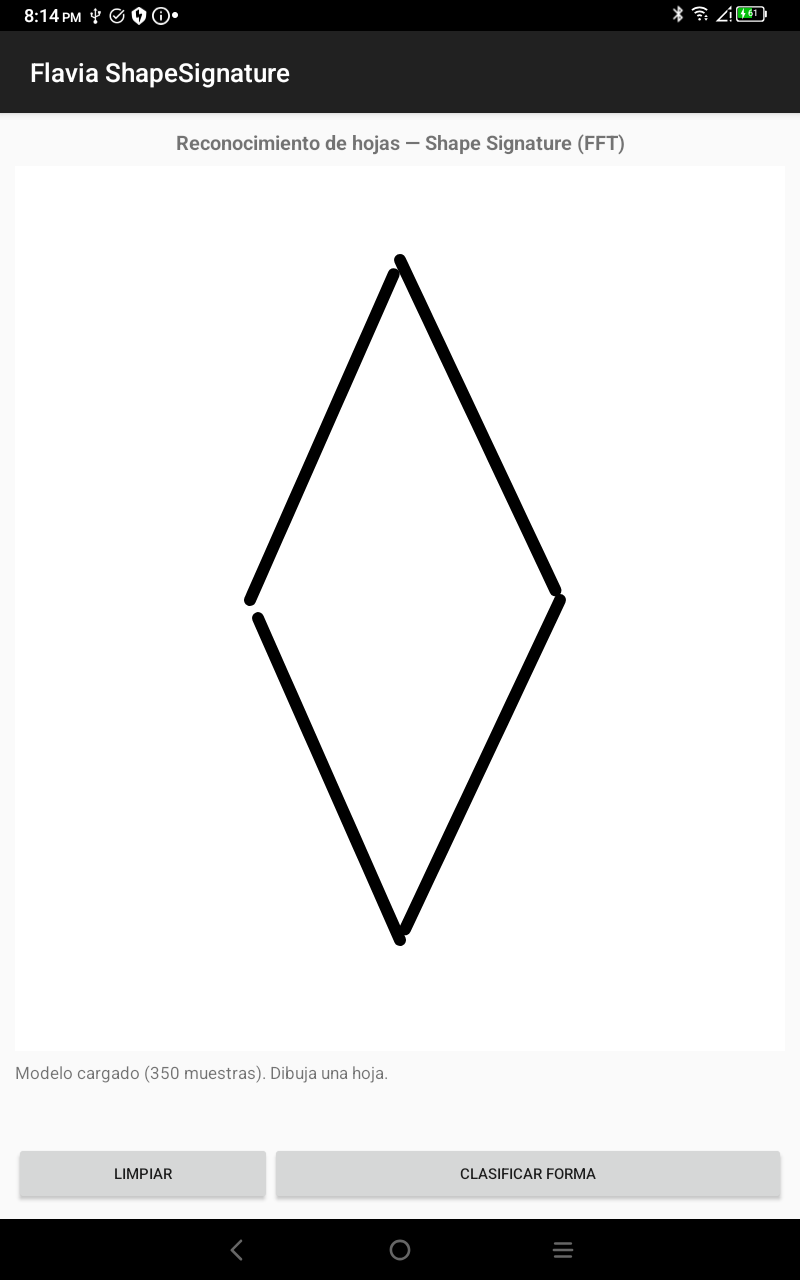
\includegraphics[width=\textwidth]{figuras/app_dibujo.png}
    \caption{Forma dibujada en el lienzo}
  \end{subfigure}
  \hfill
  \begin{subfigure}[b]{0.42\textwidth}
    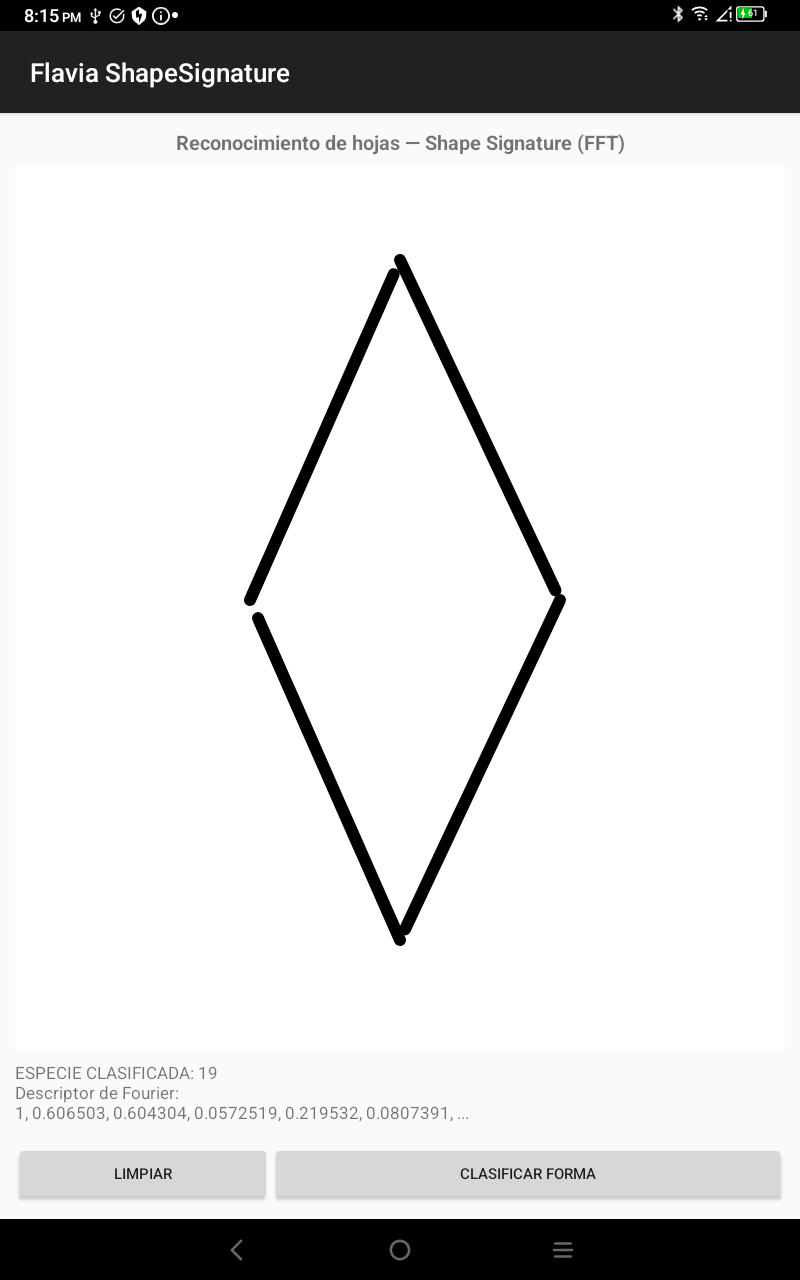
\includegraphics[width=\textwidth]{figuras/app_resultado.png}
    \caption{Resultado: ``ESPECIE CLASIFICADA: 19''}
  \end{subfigure}
  \caption{App Android ejecutándose en dispositivo real. Tras pulsar ``Clasificar forma'', el núcleo C++ calcula el descriptor de Fourier de coordenadas complejas y devuelve la especie predicha con su vector descriptor.}
  \label{fig:app}
\end{figure}

\subsection{Resultados: exactitud y formas confundidas}

Sobre el conjunto de prueba (20\% de cada clase), el sistema alcanza una \textbf{exactitud del 93.5\%}, idéntica en la implementación de Python y la de C++ (lo que confirma que el núcleo compartido es consistente). La Figura~\ref{fig:cm_p2} muestra la matriz de confusión y la Figura~\ref{fig:confundidas} algunos ejemplos de hojas que el sistema confunde.

\begin{figure}[htbp]
  \centering
  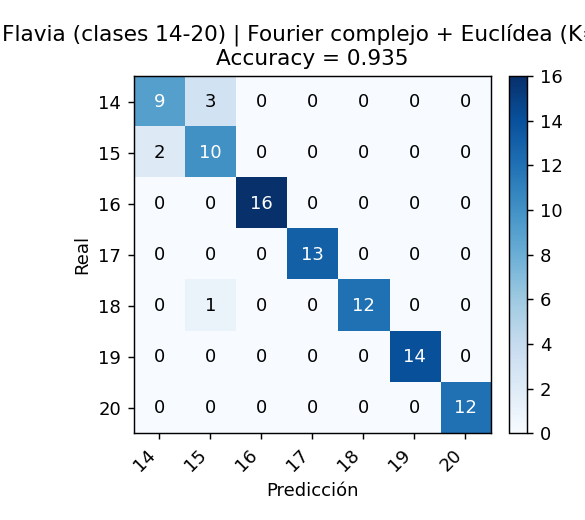
\includegraphics[width=0.6\textwidth]{figuras/confusion_matrix_part2.png}
  \caption{Matriz de confusión de las clases asignadas al G3 (14--20) sobre el conjunto de prueba. La diagonal concentra la mayoría de las predicciones (exactitud 93.5\%).}
  \label{fig:cm_p2}
\end{figure}

\begin{figure}[htbp]
  \centering
  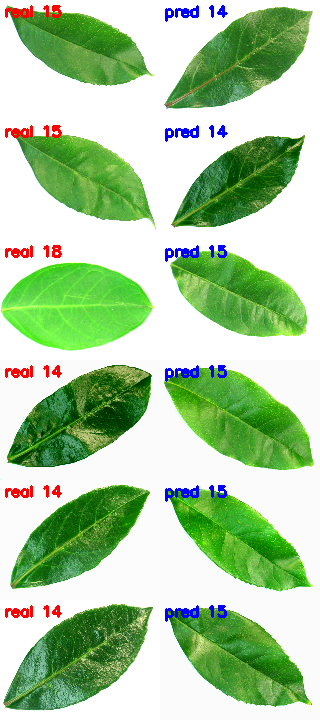
\includegraphics[width=0.32\textwidth]{figuras/hojas_confundidas.png}
  \caption{Ejemplos de hojas confundidas (real vs.\ predicha). Los errores se concentran entre las clases 14, 15 y 18, que son hojas \textbf{lanceoladas casi idénticas}: contornos alargados y simétricos cuya firma de Fourier es muy parecida.}
  \label{fig:confundidas}
\end{figure}

Las confusiones tienen una explicación razonable: las clases 14, 15 y 18 corresponden a hojas de forma lanceolada (alargadas y de bordes lisos). Como el descriptor solo usa el \textit{contorno} y descarta la textura interna y el color, dos hojas con siluetas casi iguales producen descriptores muy cercanos. Esto es coherente con la recomendación de la guía de explorar otras métricas de similitud (Manhattan, correlación) para separar clases parecidas.

% =============================================================================
\section{Conclusiones}
% =============================================================================

\begin{enumerate}

\item \textbf{La ortogonalidad sí importa.} Los Momentos de Hu se quedaron en $\sim$64\% mientras que Zernike y Shape Signature superaron el 80\% incluso con ruido alto. Hu solo aporta 7 valores muy correlacionados entre sí; las bases ortogonales y espectrales capturan más información sin redundancia, justo como anticipaba la guía.

\item \textbf{La normalización por $|F(1)|$ es frágil si el contorno está mal orientado.} El bug más difícil de la Parte 2 no fue la FFT en sí, sino que \texttt{findContours} devolvía contornos horarios que ponían el fundamental en $F(N-1)$. Forzar la orientación antihoraria fue lo que hizo que la invarianza a escala y rotación funcionara de verdad.

\item \textbf{Un solo núcleo C++ para PC y móvil ahorra muchos errores.} Compartir \texttt{shape\_descriptor.cpp} entre la CLI y la app garantizó que la exactitud medida en el PC (93.5\%) sea exactamente la que corre en la tablet, sin discrepancias por reimplementar el algoritmo dos veces.

\item \textbf{Llevar visión clásica a un móvil tiene fricción propia.} La matemática estaba lista, pero hacerla correr en la tablet exigió resolver tres problemas de integración: la imagen llega en 4 canales (RGBA), OpenCV exige STL compartida, y el lienzo de Android entrega bitmaps inmutables. Ninguno es ``visión por computador'', pero sin resolverlos la app no clasifica.

\item \textbf{El contorno no lo es todo.} El 6.5\% de error se concentra en hojas lanceoladas casi idénticas (14/15/18). Un descriptor puramente de contorno no puede distinguirlas; haría falta incorporar textura o nervadura, lo cual queda fuera del alcance de esta práctica pero marca el límite natural del método.

\end{enumerate}

% =============================================================================
\section*{Declaración de uso de herramientas de IA}
% =============================================================================

Parte de este proyecto se desarrolló con asistencia del modelo de inteligencia artificial \textbf{Claude} (Anthropic, 2026). Para ser transparentes, detallamos a continuación los componentes \textit{complicados} —los que no corresponden a una llamada directa de OpenCV ni están cubiertos paso a paso en las diapositivas— en los que se usó esta asistencia:

\begin{itemize}
  \item \textbf{Implementación desde cero de los Momentos de Zernike} ($n=8$): construcción de los polinomios radiales $R_{nm}$, la base compleja $V_{nm}$ y la proyección $A_{nm}$, con cacheo de la base para acelerar el cálculo.
  \item \textbf{Corrección de orientación del contorno} (área con signo) para estabilizar la normalización por $|F(1)|$ del descriptor de Fourier de coordenadas complejas.
  \item \textbf{Puente JNI C++$\leftrightarrow$Java} (\texttt{native\_lib.cpp}) y la configuración de CMake/Prefab para reutilizar el mismo núcleo C++ en escritorio y en Android.
  \item \textbf{Depuración en dispositivo real:} conversión de la imagen de 4 canales (RGBA) a gris (\texttt{COLOR\_BGRA2GRAY}), uso de STL compartida (\texttt{c++\_shared}) y copia mutable del bitmap del lienzo, que eran la causa de los cierres inesperados de la app.
  \item \textbf{Segmentación por envolvente convexa} de la tinta significativa para reconstruir siluetas sólidas a partir de trazos abiertos en la Parte 1.
  \item \textbf{Prevención de fuga de datos} con \texttt{GroupShuffleSplit} y la generación de las figuras y matrices de confusión.
\end{itemize}

La \textbf{teoría y la matemática} de la práctica (momentos de Hu, momentos de Zernike, firma de la forma, FFT, distancia Euclídea, KNN y PCA) se implementaron siguiendo directamente la \textit{Guía de Práctica 3-1/3-2} del docente y el material teórico de la asignatura. La IA se utilizó como apoyo de implementación y depuración, no como sustituto del razonamiento sobre los descriptores, que entendemos y podemos defender.

% =============================================================================
\section*{Referencias}
% =============================================================================

\begin{enumerate}[label={[\arabic*]}]
  \item Gonzalez, R.C., \& Woods, R.E. (2018). \textit{Digital Image Processing} (4th ed.). Pearson. \textit{[Referencia principal del curso]}

  \item Robles Bykbaev, V. (2026). \textit{Guía de Práctica de Laboratorio 3-1 / 3-2: Análisis comparativo de robustez entre Momentos de Hu y Zernike, y reconocimiento de formas mediante Firmas Espectrales con FFT de Coordenadas Complejas}. Universidad Politécnica Salesiana.

  \item Hu, M.K. (1962). Visual pattern recognition by moment invariants. \textit{IRE Transactions on Information Theory}, 8(2), 179--187.

  \item Teague, M.R. (1980). Image analysis via the general theory of moments. \textit{Journal of the Optical Society of America}, 70(8), 920--930. \textit{[Momentos de Zernike]}

  \item Zhang, D., \& Lu, G. (2004). Review of shape representation and description techniques. \textit{Pattern Recognition}, 37(1), 1--19. \textit{[Shape Signature y descriptores de Fourier]}

  \item Wu, S.G., Bao, F.S., Xu, E.Y., Wang, Y.X., Chang, Y.F., \& Xiang, Q.L. (2007). A leaf recognition algorithm for plant classification using probabilistic neural network. \textit{IEEE ISSPIT}. \textit{[Flavia Dataset]}

  \item Bradski, G., \& Kaehler, A. (2008). \textit{Learning OpenCV: Computer Vision with the OpenCV Library}. O'Reilly Media.

  \item Adolfo Gavilanes. (2024). \textit{UPS-Writing-Skills Dataset}. Kaggle. \url{https://www.kaggle.com/datasets/adolfogavilanes/ups-writing-skills}

  \item Anthropic. (2026). \textit{Claude — AI assistant}. \url{https://www.anthropic.com}. \textit{[Asistencia en implementación y depuración de componentes C++/JNI/Android no cubiertos en el material de clase]}
\end{enumerate}

\end{document}
